\documentclass[12pt, a4paper]{article}

\usepackage[utf8]{inputenc}
\usepackage{lmodern}
%\usepackage{fourier}
\usepackage{setspace}
	\singlespacing

\usepackage[frenchb]{babel}
\usepackage{xspace}
\usepackage[margin= 2.5cm]{geometry}
\pagestyle{plain}
\renewcommand{\thefootnote}{\fnsymbol{footnote}}

\usepackage{tikz}
	\usetikzlibrary{shapes}
\usepackage{graphicx}
	\graphicspath{{img/}}

\usepackage{varioref}
	\renewcommand{\reftextbefore}{page précédente}
	\renewcommand{\reftextfacebefore}{page ci-contre}
	\renewcommand{\reftextafter}{page suivante}
	\renewcommand{\reftextfaceafter}{page ci-contre}
	\renewcommand{\reftextcurrent}{}

\usepackage{amsmath, amsfonts}
\everymath{\displaystyle}


\newcommand{\espace}{\vspace{.8cm}}
\newcommand{\pg}{

}

%% REMPLIR
\usepackage[colorlinks=true, allcolors=blue, pdfborder={0 0 0}]{hyperref}
	\hypersetup{
		pdftitle={Rhénatic},
		pdfsubject={Rapport Rhénatic},
		pdfkeywords={Rhénatic, IARISS, Rapport},
		pdfauthor={IARISS Team}
	}
\title{Défi Rhénatic}
\newcommand{\authors}{Florent}

%
\begin{document}

\author{
\includegraphics{../_img/iariss_team.png} \\ {\sffamily \href{http://iarissteam.me}{iarissteam.me}}}
\date{\today}

\maketitle{}

{\sffamily Ce rapport a pour but de montrer dans quel mesure notre application peut-être fun et surprenante !} 

\espace{}
\section*{Notre application}
Nous avons voulu développez une application qui parait très simple pour l'utilisateur, bien que le moteur derrière soit bien plus compliqué : lé simplicité dans la complexité ! Tout ce que l'utilisateur a à faire, c'est d'entrer quelques mots clés dans le champ de recherche, et de cliquer sur valider. Il peut ensuite naviguer entre différents thèmes, villes, époque,\ldots{} et ceux en toute simplicité grâce à notre système de tag ! Le but de notre site est que l'utilisateur trouve une réponse le plus rapidement possible.

De plus, nous avons caché deux easter eggs dans notre applications, en rapport avec le thème alsaco-canadien demandé par l'un des défis.
Pour découvrir le premier, il suffit d'entrer le \href{http://fr.wikipedia.org/wiki/Code_Konami}{code Konami}, c'est à dire la combinaison de touche haut haut bas bas gauche droite gauche droite B A.
Pour de deuxième, il suffit de taper dans la fenêtre du navigateur la chaine de caractère \og{}je suis un caribou\fg{}, et d'attendre de voir ce qu'il se passe !
Sans oublier le thème Alsaco-Canadien !
See & enjoy !
\espace{}
\begin{center}
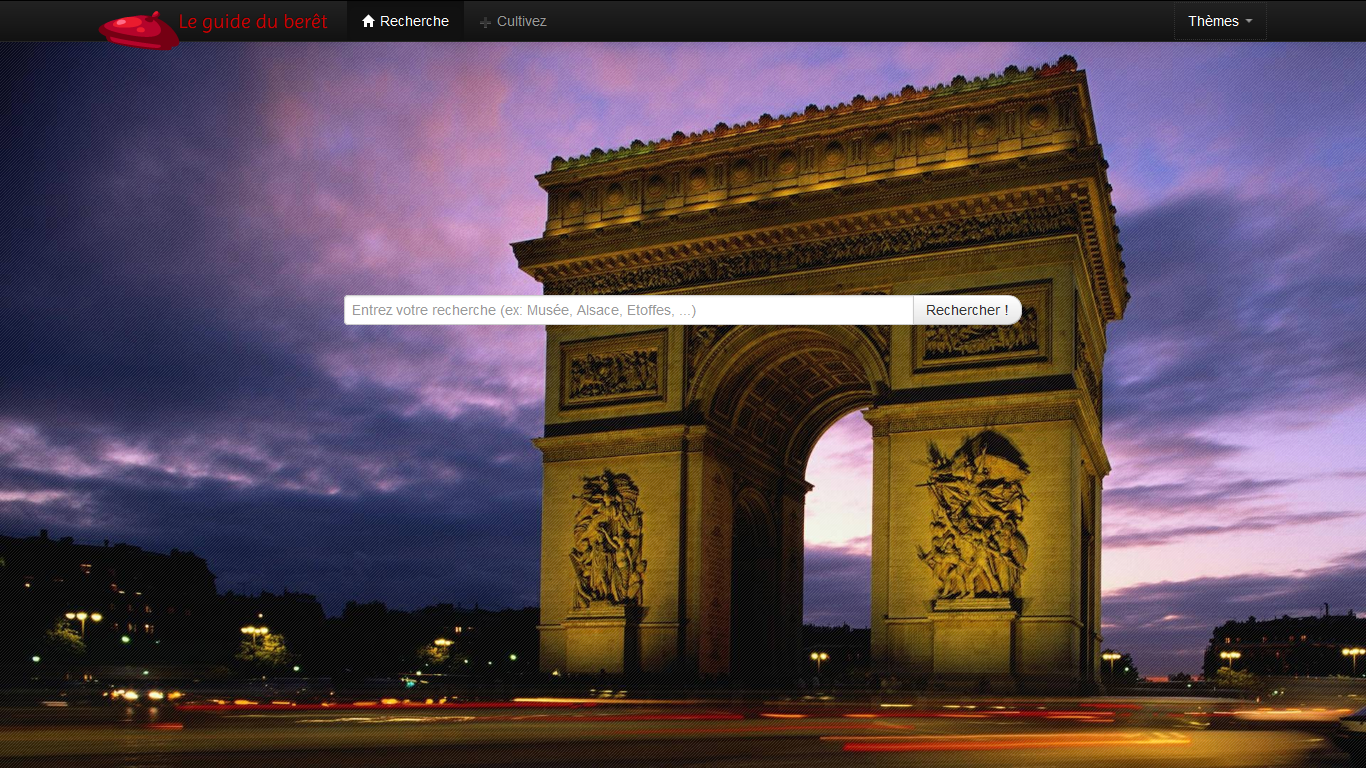
\includegraphics[width=.9\textwidth, keepaspectratio=true]{img/accueil.png}
\end{center}
\espace{}

\section*{Le reste !}
- Nous avons procédé à la mise en place d'un compte à rebours avant le début de la nuit de l'info (d'abord avec une actualisation hebdomadaire, puis ensuite un vrai décompte à partir de H-1, seconde par seconde), puis avant la fin de la Nuit de l'Info (en fond de notre \href{http://iarissteam.me/}{portail}).

- Un live a été diffusé (\href{http://live.iarissteam.me/}{http://live.iarissteam.me/}) dès le début de la nuit, et pendant toute la durée de celle-ci. Cela a impliqué la réservation préalable d'un nom de domaine.

- Une seconde webcam a été mis ene place en parallèle dans le but de réaliser un timelapse (disponible \href{ici}{ici}). A partir de 14h et jusqu'à la fin de la nuit, une photo a été prise toute les secondes. Toutes ces images ont ensuite été résumé dans une vidéo résumant la Nuit de l'Info, en accéléré.

- Enfin, un tumblr \href{http://lesjoiesdelanuit.tumblr.com/}{Les Joies de la Nuit} (inspiré de \href{http://lesjoiesducode.tumblr.com/}{Les joies du Code}), avec tweet automatique pour chaque nouvel article posté. Ce tumblr a été alimenté touteau long de la nuit, par des articles préparées à l'avance, mais aussi en \og{}live\fg{}, en fonction des différents évènements arrivés au cours de la nuit. Voici un court extrait ci-après : 

\espace{}
\begin{center}
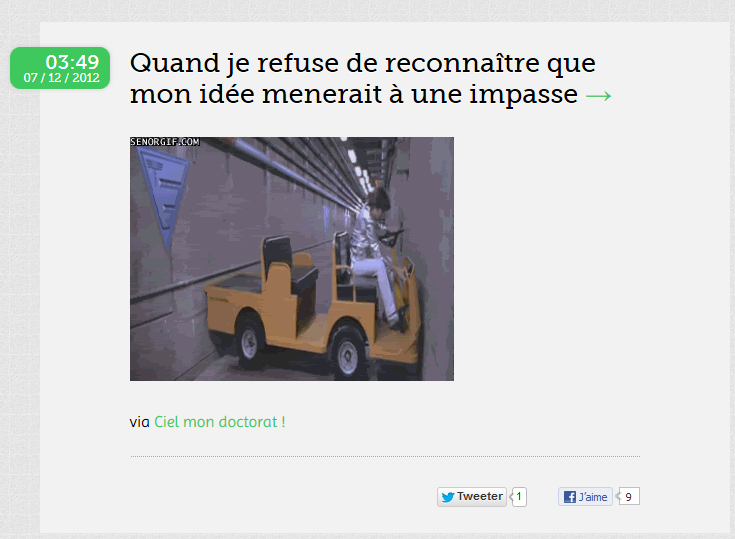
\includegraphics[width=.9\textwidth, keepaspectratio=true]{img/tumblr.png}
\end{center}
\espace{}



%\espace{}
%\begin{figure}[h]
%	\begin{center}
%	\end{center}
%	\caption{\label{fig-} Légende}
%\end{figure}

\espace\vfill{}
Ce document a été rédigé en \LaTeX{} par \authors{} pour IarissTeam avec quelques tasses de café et beaucoup de bonne humeur.

Contactez-nous à \href{mailto:nuitinfo@iariss.com}{nuitinfo@iariss.com} pour tout renseignement supplémentaire !

\end{document}